\documentclass{standalone}

\usepackage{blox}
\usepackage{tikz}
\usepackage{amsmath}  % For math
\usetikzlibrary{positioning}
\newcommand{\equal}{=}
\usepackage{tikz}



\begin{document}

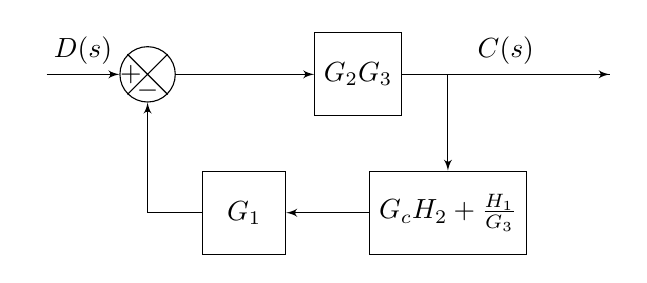
\begin{tikzpicture}
\bXInput{A}
\bXComp{B}{A}
\bXLink[$D(s)$]{A}{B}
\bXChain[5]{B}%
{G2G3/$G_2G_3$}
\bXOutput[7.5]{E}{G2G3}
\bXLink[$C(s)$]{G2G3}{E}
\bXBranchy[5]{E}{returnDown}

% return loop
\bXBlocr[3]{GcBlock}{$G_cH_2+\frac{H_1}{G_3}$}{returnDown}
\bXBlocr[3]{G1}{$G_1$}{GcBlock}
\bXLink{GcBlock}{G1}
\bXLinkxy{G1}{B}
\bXLinkxy{E}{GcBlock}
%\bXReturn{G3-E}{B}{}
\end{tikzpicture}

\end{document}